\documentclass[12pt,openright,oneside,a4paper,brazil]{abntex2}
\usepackage[utf8]{inputenc}
\counterwithout{section}{section}
\counterwithout{figure}{chapter}
\counterwithout{table}{chapter}
\setlength{\parindent}{1.3cm}
\usepackage{indentfirst}
\setlength{\parskip}{0.2cm}
\usepackage[bottom=2cm,top=3cm,left=3cm,right=2cm]{geometry}
\usepackage{graphicx}
\graphicspath{{figuras/}}
\usepackage{placeins}

%opening
\title{}
\author{}

\begin{document}


\textual
\begin{center}
 {\large Plano de gerenciamento de Qualidade}\\[0.2cm]
 {Planta de abastecimento de água potável a partir da umidade do ar}\\
 \end{center}
 
 \section{Histórico de Alterações}
\begin{table}[h]
\centering
\begin{tabular}{|c|c|p{6cm}|p{5cm}|}

Data & Versão & Descrição & Responsável\\
\hline                               
19/04/2015 & 0.0 & Criação do Plano de Gerenciamento de Qualidade & Alexandre T. Kryonidis, André Luis, Matheus Jericó\\
\hline
20/04/2015 & 1.0 & Revisão do Plano & Alexandre K., André Luis.\\
\hline
\end{tabular}
\end{table}

\section{Objetivo}
  O objetivo desse plano é estabelecer um processo de gerenciamento e controle da qualidade do projeto.
  
\section{Descrição dos processos de gerenciamento da qualidade}
 A qualidade de um projeto está relacionada, principalmente, com o cumprimento dos requisitos levantados, ou seja, satisfaz os objetivos a que o projeto se propôs a solucionar. Dessa forma pretende-se gerenciar a qualidade do projeto da seguinte maneira:
 \begin{itemize}

\item As alterações nos requisitos de qualidade previstos para o sistema devem passar por uma avaliação do sistema de controle de mudanças da qualidade.
\item Todas as reclamações provenientes dos stakeholders serão avalidadas e, ao corrigi-las, deverão ser tratadas como medidas corretivas no plano de gerenciamento da qualidade.
\item Todos os produtos ou entregas que não cumprem obedecem a declaração de escopo deverão ser tratadas como medidas corretivas no plano de gerenciamento de qualidade.
\item As solicitações de mudanças devem ser documentadas de acordo com o plano de comunicações do projeto.	
 \end{itemize}
 
 \section{Priorização das mudanças nos quesitos de qualidade e respostas}
 \begin{itemize}
 \item Prioridade Alta
 
 Mudanças de alta prioridade causam um grande impacto no projeto e deverão ser tratadas em caráter de urgência, pelo gerente do Projeto, em conjunto com algum membro da equipe de qualidade. Essas mudanças devem ser abordadas durante as  reuniões de grupos apesar delas serem independentes das reuniões de controle, devido ao seu grau de importância. 
 
 \item Prioridade Média
 
 Mudanças de média prioridade envolvem um impacto que requer ação rápida do Gerente de Projeto, também em conjunto com a equipe de qualidade. Podem ser tomadas antes das reuniões de controle, mas também é possivel esperar um pequeno prazo para serem avaliadas por um número maior de “steakholders”. Os resultados dessa mudança também devem ser debatidos nas reuniões.

\item Prioridade Baixa

	Mudanças de prioridade Baixa não acarretam alterações significativas na elaboração do projeto e, portanto, não é requerida uma ação imediata, está dentro da autonomia de qualquer integrante da gerencia do Projeto
 \end{itemize}
 
 \section{Sistema de controle de mudanças da qualidade}
 As realizações do controle de qualidade das entradas, que passaram por solicitações de mudanças devem ser verificadas, podendo ocorrer modificações como reparo de defeitos, revisão dos métodos de trabalho e revisão do cronograma. Nas saídas, os itens alterados ou reparados são inspecionados e serão aceitos ou rejeitados antes do fornecimento. Os rejeitados podem exigir retrabalho.
 \begin{figure}[h]
 \begin{center}

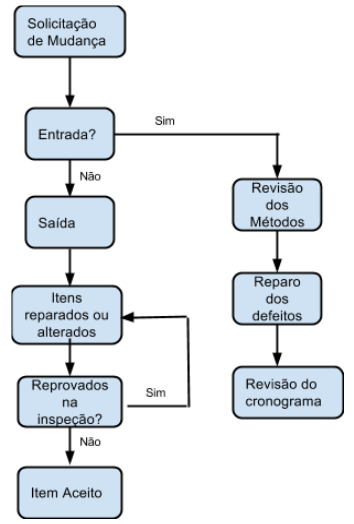
\includegraphics[scale=0.6]{mudanca}
\label{Mudanca}
 \end{center}
 \end{figure}
 \FloatBarrier
 
 \section{Frequência de avaliação dos requisitos de qualidade do projeto}
 Os requisitos de qualidade serão avaliados e, caso necessário, atualizados de duas em duas semanas. Os resultados obtidos a partir das análises relacionados a qualidade do projeto serão apresentados nas reuniões presenciais do grupo.

\section{Alocação financeira das mudanças nos requisitos de qualidade}
Todas as mudanças a serem efetuadas devem entar dentro do previsto pela equipe de gerenciamento de custo, qualquer alteração que impacte no orçamento do projeto, será discutida com os reponsáveis pelo custo. Como não temos patrocinadores nesse momento, não teremos formas de adquirir novos recursos com facilidade, por isso, gastos adicionais devem ser evidados. Porém, se esse gasto adicinal trouxer beneficios consideráveis para o projeto não deverá ser descartado. Qualquer necessidade de avaliação de custos será atribuida a equipe de gerenciamento de custo, ou estará sujeita a  análise e aprovação pela mesma.

\section{Administração do plano de gerenciamento da qualidade}
\begin{enumerate}
\item Responsável pelo plano:
\begin{itemize}
\item Alexandre Torres Kryonidis - Gerente de qualidade.
\item André Luis - suplente do responsável pelo plano de gerenciamento de qualidade.
\end{itemize}
\item	Freqüência de atualização do plano de gerenciamento da qualidade

O plano de qualidade será avaliado quinzenalmente e, caso necessário, será atualizado após essas avaliações. Qualquer necessidade de alteração no plano antes desse periodo, deverá ser tratado segundo os procedimentos tratados no item IX (Outros assuntos relacionados ao gerenciamento da qualidade do projeto não previstos neste plano)
\end{enumerate}

\section{Outros assuntos relacionados ao gerenciamento da qualidade do projeto não previstos nesse plano}
Qualquer solicitação que não se enquadrem nos preceitos deste plano deverão ser abordados nas reuniões semanais de acompanhamento do projeto, desse forma, serão dados os devidos encaminhamentos. Após as aprovações, o plano de gerenciamento será atualizado com os devidos registros.
\section{Assinaturas}
\begin{center}
Data: \rule{0.5cm}{0.1mm}/\rule{0.5cm}{0.1mm}/\rule{1cm}{0.1mm}     \\
\rule{13cm}{0.1mm}\\
ADRIANNY VIANA DE ARAÚJO AMORIM – GERENTE DE PROJETO\\
\rule{13cm}{0.1mm}\\
ALEXANDRE TORRES KRYONIDIS - GERENTE DE QUALIDADE

\end{center}
\end{document}